% ECTEL 2026 - Full Research Paper
% paper2.tex — revised version
%
\documentclass[runningheads]{llncs}
%
\usepackage[T1]{fontenc}
\usepackage{graphicx}
\usepackage{amsmath, amsfonts, amssymb}
\usepackage{tabularx}
\usepackage{booktabs}
\usepackage{hyperref}
\usepackage[markup=underlined, authormarkup=none]{changes}
\usepackage{subcaption}
\usepackage{float}
\definechangesauthor[name=Development, color=blue]{dev}
%
\graphicspath{{img/}}
%
\begin{document}
%
\title{Augmented User Modeling via Grounded Transformers}
%
\titlerunning{Augmented User Modeling via Grounded Transformers}
%
\authorrunning{}
%
\institute{}
%
\maketitle
%
\begin{abstract}

Intelligent Tutoring Systems (ITS) rely on student models to drive adaptive instruction, yet the Knowledge Tracing approaches that underpin these models have been developed almost exclusively to optimise predictive accuracy. The resulting representations are either interpretable but rigid, as in classical Bayesian Knowledge Tracing (BKT), or accurate but opaque, as in deep knowledge tracing models. Neither type produces actionable outputs that educators can inspect, validate, or act upon directly. While recent work has proposed \textit{representational grounding} as a design principle for interpretable deep knowledge tracing, it has not addressed how the resulting theory-grounded parameters can be integrated into an ITS to support purposeful instructional decisions. The present paper addresses this gap by contributing the design of an \textit{augmented student model} that translates the outputs of such grounded models into instructionally actionable representations. Specifically, we show how continuously updated estimates of prior knowledge and learning rate can be used to assign each student to one of four \textit{learning situations}, defined by a data-driven partition of the parameter space, and how each situation implies a distinct and evidence-grounded instructional strategy. The result is a student-centred design in which pedagogically-grounded instructional strategies are continuously adapted to the evolving needs of each learner, with transparency and educator agency as first-class concerns.

\keywords{deep knowledge tracing \and theory-based interpretability \and grounded transformers \and user modeling \and learning theories \and intelligent tutoring systems}
\end{abstract}
%
%
\section{Introduction}

Student models are the cognitive foundation of Intelligent Tutoring Systems (ITS): they estimate the learner's evolving state of mastery and supply the information from which the tutorial model selects instructional strategies. In most deployed systems, this estimation is driven by Knowledge Tracing (KT) approaches, ranging from Bayesian Knowledge Tracing (BKT)~\cite{corbett1994knowledge} to deep knowledge tracing architectures that evolved from early recurrent neural network models such as DKT~\cite{piech2015deep} to more recent attention-based Transformer architectures~\cite{ghosh2020context}. The development of KT has been shaped almost exclusively by the objective of maximising predictive accuracy, with little regard for whether model outputs are interpretable or actionable by end users, in particular educators and instructional designers. This creates a fundamental tension: a student model whose internal representations bear no correspondence to pedagogically recognisable constructs, offers limited diagnostic value even when its accuracy is high.

Two structural limitations persist across the KT landscape. First, high-performance deep learning approaches are largely opaque: their internal states do not map to constructs that practitioners can inspect, validate or explain. Second, interpretable models such as standard BKT operate at the population level, estimating a single parameter set for all students on a given skill~\cite{yudelson2013individualized}, and therefore cannot capture the individual learning dynamics that determine which instructional strategy will be most effective for a given learner at a given moment.

A recent line of work proposes \textit{representational grounding} as a design principle for interpretable deep knowledge tracing~\cite{labra2026theory}. It shows how, by constraining a Transformer's latent representations to align with the semantic axes of a intrinsically interpretable reference model such as BKT, we can derive student-specific, longitudinally updated estimates of prior knowledge and learning rate parameters from each student's full interaction history. The work demonstrates that gTransformer, the proposed grounded model, is both valid and competitive but it doesn't address \emph{how} the resulting interpretable parameters could be integrated into an ITS to support adaptive instruction in practice.


The present paper addresses this gap. Following the conceptual framework introduced in~\cite{labra2026theory}, we adopt pedagogical grounding in established learning theory, transparency, and educator agency as guiding design principles for an augmented student model. Our contribution is the design of an \textit{augmented student model} that operationalises grounded Transformer outputs into instructionally actionable representations, enabling educators to identify distinct learning situations and adapt instruction accordingly. This design draws on BKT as its theoretical reference, ensuring that model outputs correspond to pedagogically recognised constructs, and foregrounds human judgment over automated decision-making.

The research question that guides this work is: how can augmenting an ITS user model with grounded Transformer parameters support the design of context-aware, situation-based instructional strategies that are both grounded in established learning theories and responsive to the evolving needs of individual learners?

The remainder of the paper is organised as follows. Section~2 formalises the proposed augmented user model and the gTransformer architecture that powers it, and makes explicit the design principles that govern its construction. Section~3 describes the methodology for augmenting the user model and deriving learning situations from grounded parameters. Section~4 presents the results for each learning situation and their instructional implications. Section~5 demonstrates situation-based instructional routing. Section~6 discusses the broader implications and Section~7 concludes.

\subsection{Intelligent Tutoring Systems and User Models}

Intelligent Tutoring Systems are typically structured around three interacting components:

\begin{itemize}
    \item \textit{Domain model}: This component encodes the knowledge to be taught, typically structured as a set of Knowledge Components (KCs) or skills. It provides the base through which student performance is assessed and instructional content is organised.
    \item \textit{User model}: The user model tracks the learner's evolving state by maintaining a representation of their mastery across the domain model.
    \item \textit{Tutorial model}: This component mediates instructional decisions by selecting the next activity, intervention, or level of support based on the current state of the user model. The goal is to provide a personalised learning experience that adapts to the student's trajectory.
\end{itemize}

\subsection{Learning Theories and Bayesian Knowledge Tracing}

We select BKT~\cite{corbett1994knowledge} as our reference theoretical framework. BKT models the learning process as a Hidden Markov process governed by four interpretable parameters: Initial Mastery ($P(\text{L}_0)$), the probability that a student knows a concept prior to practice; Learn Rate ($P(\text{T})$), the probability of transitioning from the unlearned to the learned state; Guess ($P(\text{G})$), the probability of a correct response despite lack of mastery; and Slip ($P(\text{S})$), the probability of an incorrect response despite mastery. These parameters enable a recursive, causally transparent estimation of student mastery that is directly interpretable by educators.

Standard BKT suffers from a significant limitation: it operates at the population level, estimating a single parameter set for all students on a given skill~\cite{yudelson2013individualized}. As a result, two students with identical recent response patterns receive the same mastery estimate and the same instructional routing, regardless of differences in their prior knowledge or in the rate at which they have been consolidating knowledge across earlier interactions. The augmented student model proposed here overcomes this limitation by replacing population-level parameter estimates with student-specific, longitudinally sensitive ones derived by gTransformer.

%
\section{Grounded Transformers and Augmented User Models}

\subsection{Proposed Architecture}

We propose an \textit{augmented user model} that integrates the three standard ITS components with a Grounded Transformer engine. The \textit{domain model} defines the structured knowledge components to be mastered. The \textit{user model} tracks student mastery across these components and is augmented with student-specific parameters $(p_{\text{L}_0}, p_{\text{T}})$ inferred by gTransformer~\cite{labra2026theory} from the student's full interaction history. These parameters encapsulate the student's longitudinal learning context, allowing the user model to differentiate learners who show similar correctness patterns but differ in prior knowledge or learning rate. The outputs of this augmented user model feed: 1)~the \textit{tutorial model}, which selects situation-based instructional strategies; and 2)~a \textit{diagnostic roster module}, which visualises student trajectories in $(p_{\text{L}_0}, p_{\text{T}})$ space to support educator oversight.

\subsection{gTransformer}

The augmented user model is powered by gTransformer~\cite{labra2026theory}, a hybrid architecture that implements representational grounding: a methodology that anchors Transformer latent representations to the semantic constructs of BKT, bridging deep learning expressiveness with pedagogical interpretability. Figure~\ref{fig_arch} summarises the architecture.

\begin{figure}[H]
\centering
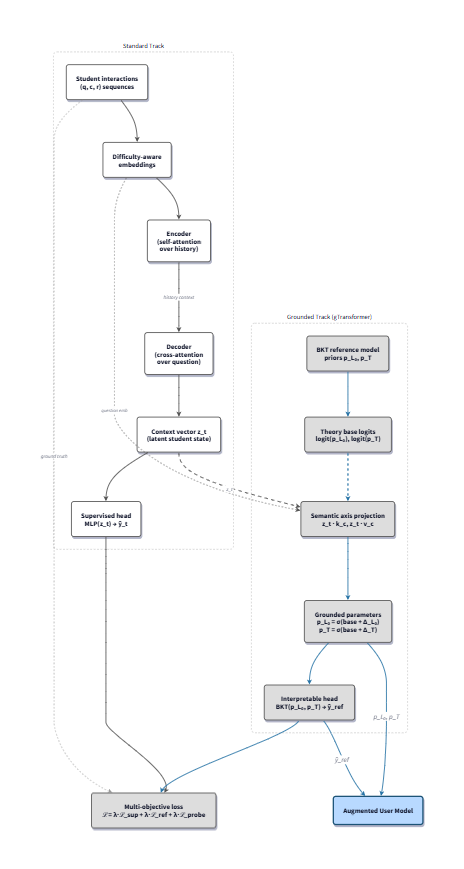
\includegraphics[width=0.65\textwidth,height=0.75\textheight,keepaspectratio]{gtransformer.png}
\caption{\textbf{gTransformer architecture.} Two processing tracks share a common encoder--decoder backbone. The standard track (white boxes) produces supervised predictions via an MLP head. The grounded track (grey boxes) combines BKT theory base logits with context-vector projections onto learnable semantic axes to produce student-specific parameters $(p_{\text{L}_0}, p_{\text{T}})$, which are passed through BKT update logic to yield theory-transparent predictions. Both heads are jointly optimised via a multi-objective loss. Outputs of the grounded track populate the augmented user model (blue box).}
\label{fig_arch}
\end{figure}

As illustrated in Figure~\ref{fig_arch}, the architecture operates through two parallel tracks. The \textit{standard track} encodes student interactions $(q_t, c_t, r_t)$ via difficulty-aware embeddings and processes them through a stacked attention-based encoder--decoder, producing a context vector $z_t$ that summarises the student's current learning state. A multi-layer perceptron maps $z_t$ directly to a correctness prediction $\hat{y}_t$, optimising for predictive accuracy without theoretical constraints.

The \textit{grounded track} implements representational grounding by composing student-specific BKT parameters in logit space. For each knowledge component, logit-transformed population-level BKT priors serve as theory base values; contextual adjustments are obtained by projecting $z_t$ onto learnable concept-specific semantic axes for initial mastery and learning rate. The resulting grounded parameters $p_{\text{L}_0,t} = \sigma(\ell_{\text{L}_0} + z_t \cdot k_c)$ and $p_{\text{T},t} = \sigma(\ell_{\text{T}} + z_t \cdot v_c)$ are passed through BKT update logic to produce interpretable predictions $\hat{y}_{\text{ref},t}$. Training is governed by a multi-objective loss balancing supervised accuracy, interpretable prediction quality, and global latent-space alignment through diagnostic probing. Full architectural details are provided in~\cite{labra2026theory}.

\subsection{Design Principles}

The augmented student model presented here is shaped by three explicit design principles, each of which traces directly to a concrete implementation decision. Making this traceability visible is central to the ECTEL theme of Mindful TEL: a technology shaped with intention must be able to account for why it was designed the way it was, including what it deliberately does not do.

\textbf{Interpretability as a first-class requirement.} Rather than relying on post hoc explanation techniques such as attention weight visualisation, the system produces outputs that are intrinsically grounded in BKT parameters. This choice limits the model to the parameter space defined by a well-established learning theory but ensures that every prediction can be traced to constructs that educators recognise and can validate. Raw model internals are not surfaced to practitioners.

\textbf{Transparency toward educators.} The grounded parameters $(p_{\text{L}_0}, p_{\text{T}})$ and their derived learning situations are designed to be readable by non-specialist practitioners. The four learning situation labels (foundational, emerging, consolidating, advancing) map to observable learning patterns and imply concrete instructional actions, rather than encoding latent scores that require technical expertise to interpret.

\textbf{Educator agency over automation.} The model does not issue automated instructional recommendations or select content without human involvement. It provides educators and the tutorial model with structured, theory-grounded evidence about each student's current learning situation. Instructional decisions remain with the practitioner. This is a deliberate constraint: rather than maximising automation, the design preserves the capacity for human judgment and oversight, which is required for responsible deployment of AI in high-stakes educational contexts~\cite{Holmes2022504}.

%
\section{Methodology}

Our methodology operationalises the research question by augmenting the ITS user model with the grounded parameters produced by gTransformer and demonstrating how these parameters enable situation-based instructional routing. The validation proceeds along two lines.

\subsection{Augmenting the User Model}

For each student $s$ and knowledge component $c$, gTransformer infers a pair of longitudinally updated parameters $(p_{\text{L}_0,t}, p_{\text{T},t})$ from the full interaction sequence up to time $t$. These are not population-level constants: they are student- and context-specific estimates that encode how much prior knowledge the student brings to a given skill and at what rate new knowledge is being consolidated. They are produced by the grounded track of gTransformer (Section~2.2) and passed through BKT update logic to generate interpretable predictions $\hat{y}_{\text{ref},t}$.

To augment the user model, we record the most recent $(p_{\text{L}_0}, p_{\text{T}})$ pair for each student alongside the standard mastery estimate. This extended user profile allows the ITS to distinguish students who show similar response patterns but differ in their underlying learning dynamics, a distinction that population-level BKT cannot make. We validate the quality of this augmented user model by comparing $\hat{y}_{\text{ref}}$ against classical BKT predictions using AUC on the ASSISTments 2009 (AS2009) dataset.

\subsection{Clustering into Learning Situations}

To translate the continuous parameter space into actionable instructional decisions, we partition the $(p_{\text{L}_0}, p_{\text{T}})$ plane into four \textit{learning situations} using the population medians of both parameters as thresholds. This yields a $2 \times 2$ partition that is interpretable, non-parametric, and data-driven. The partition is intentionally coarse: finer-grained segmentation would reduce the interpretability of the resulting labels and obscure the correspondence to pedagogically meaningful instructional strategies. The four situations are:

\begin{itemize}
    \item \textit{Foundational} (low $p_{\text{L}_0}$, low $p_{\text{T}}$): limited prior knowledge and a slow consolidation rate. The instructional priority is scaffolding: worked examples, reduced problem complexity, and frequent low-stakes retrieval practice to establish a stable knowledge base before progressing.
    \item \textit{Emerging} (low $p_{\text{L}_0}$, high $p_{\text{T}}$): limited prior knowledge but a high learning rate. The situation calls for targeted practice on weaker knowledge components while progressively increasing challenge; the high consolidation rate means well-designed instruction can produce rapid gains.
    \item \textit{Consolidating} (high $p_{\text{L}_0}$, low $p_{\text{T}}$): substantial prior knowledge but a low marginal learning rate, indicating that current instructional conditions are no longer generating new knowledge. The tutorial model should introduce cross-domain challenge or novel problem types to reactivate the learning trajectory.
    \item \textit{Advancing} (high $p_{\text{L}_0}$, high $p_{\text{T}}$): high prior knowledge combined with an active learning rate. These students can be routed to accelerated content, reduced practice redundancy, and higher-order reasoning tasks without risk of premature challenge.
\end{itemize}

Because gTransformer updates $(p_{\text{L}_0,t}, p_{\text{T},t})$ at every interaction, a student's assigned learning situation is not fixed at enrolment: it is a rolling summary of their current longitudinal profile, and the tutorial model updates its routing whenever the parameter pair crosses a quadrant boundary. This dynamic routing is the core mechanism through which the augmented user model supports situation-based instruction. The four labels are descriptions of observable learning patterns, not fixed categories or fixed student characteristics.

%
\section{Results}

Augmenting the user model with grounded Transformer parameters yields a measurable gain in predictive accuracy: interpretable predictions derived from gTransformer consistently outperform classical BKT, with an average AUC gain of 19.9\% on the AS2009 dataset. This validates that context-aware, student-specific parameters capture the nuances of individual learning journeys while remaining within the interpretable framework of BKT.

Figure~\ref{fig_roster} addresses the second line of validation by showing trajectory plots for the representative student of each learning situation on the AS2009 dataset. Each panel traces consecutive sampled interactions in the $(p_T, p_{L_0})$ plane. The representative for each quadrant is the student who maximises a composite score balancing proximity to the quadrant centroid and number of interactions (equal weights). A candidate point is sampled every 5 interactions and retained only when its Euclidean distance from the last plotted point exceeds $\delta_{\min}\approx 0.3$; otherwise it is absorbed into the preceding point, whose marker area grows proportionally to encode dwell time. The $p_T$ axis is capped at 0.5 to exclude a small fraction of high-rate outlier interactions ($<$6\%). The first and last directional arrows are rendered in a darker tone to temporally anchor the trajectory; all intermediate arrows are in light grey. Coloured background regions delimit the four learning situations; a point may cross boundaries, indicating a genuine shift over time.

The four trajectories are qualitatively distinct in ways that are directly instructionally informative. The \textit{foundational} student (120 interactions, 8 plotted points) remains anchored in the lower-left quadrant throughout, with transient fluctuations that consistently return to low mastery and low learning rate, indicating that current instructional conditions are insufficient to drive durable progress. The \textit{consolidating} student (148 interactions, 3 plotted points) yields the most compact trajectory of all four: the large marker at the terminal point (interaction 25) encodes the 123 subsequent interactions that produced no displacement exceeding $\delta_{\min}$, making the prolonged absence of movement the primary visible signal of stagnation rather than the parameter values themselves. The \textit{emerging} student (156 interactions, 15 plotted points, after excluding a small fraction of high-rate outliers with $p_T > 0.5$) produces the most spatially extended orbit, crossing all four quadrants; both $p_{L_0}$ and $p_T$ oscillate with large steps across a wide portion of the visible range, making parameter variability the defining feature of this trajectory rather than convergence to a stable attractor. The \textit{advancing} student (168 interactions, 4 plotted points) shows consistently high prior mastery combined with above-median learning rates throughout; the large marker at the final plotted point encodes the remaining interactions, confirming that the parameter pair stays in the upper-right region for the bulk of the trajectory. By reading these trajectories, educators gain theory-grounded evidence of whether a student is disengaging (decreasing $p_{\text{T}}$), stagnating (stable high $p_{\text{L}_0}$, falling $p_{\text{T}}$), or actively learning (increasing parameters, boundary crossings); evidence that supports intentional instructional decision-making and satisfies the accountability requirements for high-risk educational AI.

\begin{figure}[H]
\caption{\textbf{Learning situation trajectories.} Each plot traces the evolution of the parameter pair $(p_T, p_{L_0})$ for the representative student of one learning situation in the AS2009 dataset. Marker area encodes dwell time (interactions absorbed between two plotted points). The first and last arrows are rendered in a darker tone; all intermediate arrows are in light grey. The $p_T$ axis is capped at 0.5. Coloured background regions delimit the four learning situations.}
\label{fig_roster}
\centering
\begin{subfigure}[b]{\textwidth}
  \centering
  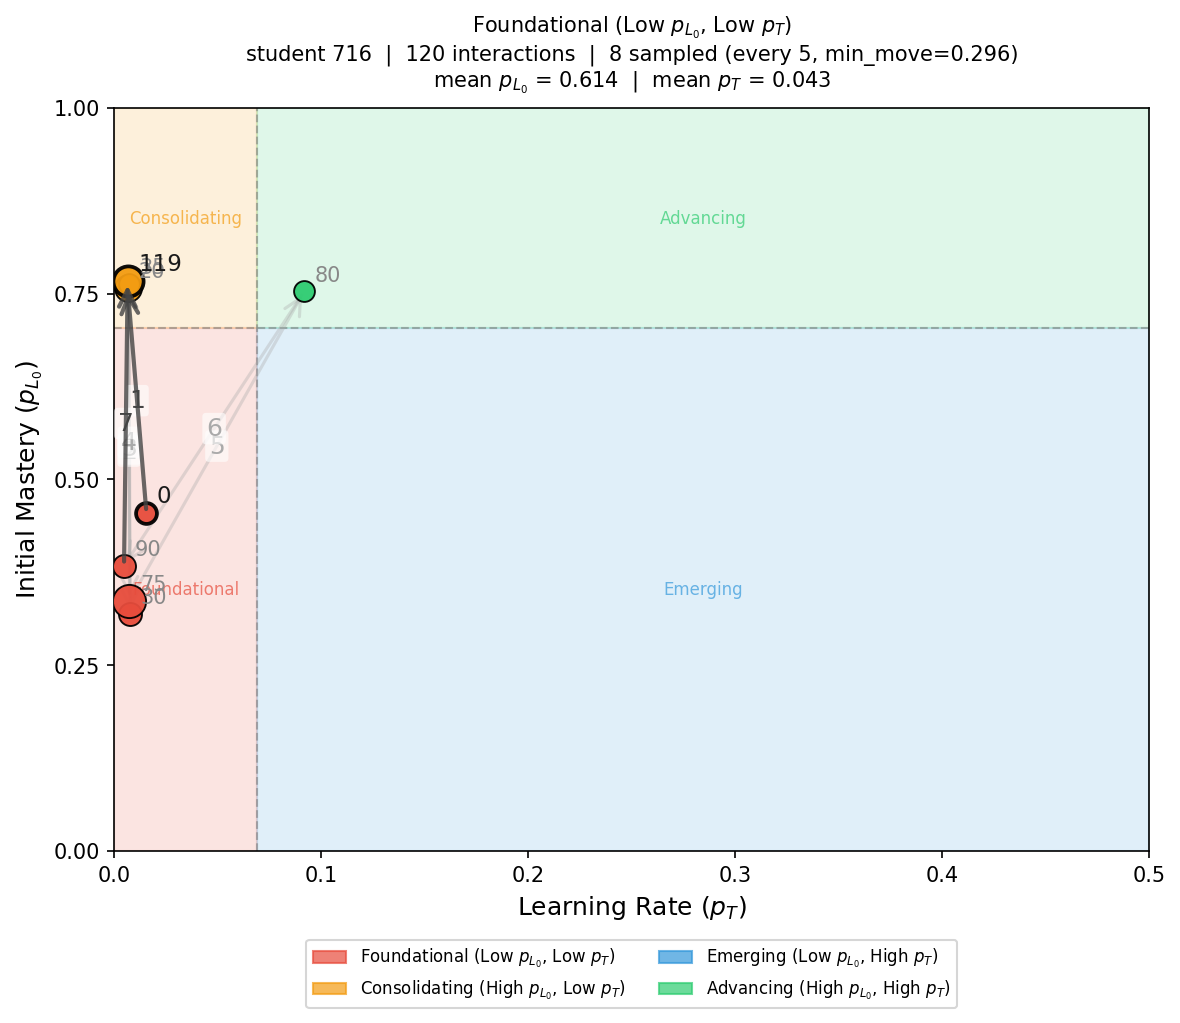
\includegraphics[width=0.8\textwidth,height=0.36\textheight,keepaspectratio]{roster_2d_foundational_893468.png}
  \caption{\textit{Foundational} (low $p_{L_0}$, low $p_T$): 8 points plotted across 120 interactions. The trajectory remains anchored in the lower-left quadrant throughout, with transient fluctuations that quickly return to low mastery and low learning rate. The compact spread and persistent low $p_T$ suggest that current instructional conditions are insufficient to drive durable progress, signalling a need for scaffolding and worked examples.}
\end{subfigure}
\begin{subfigure}[b]{\textwidth}
  \centering
  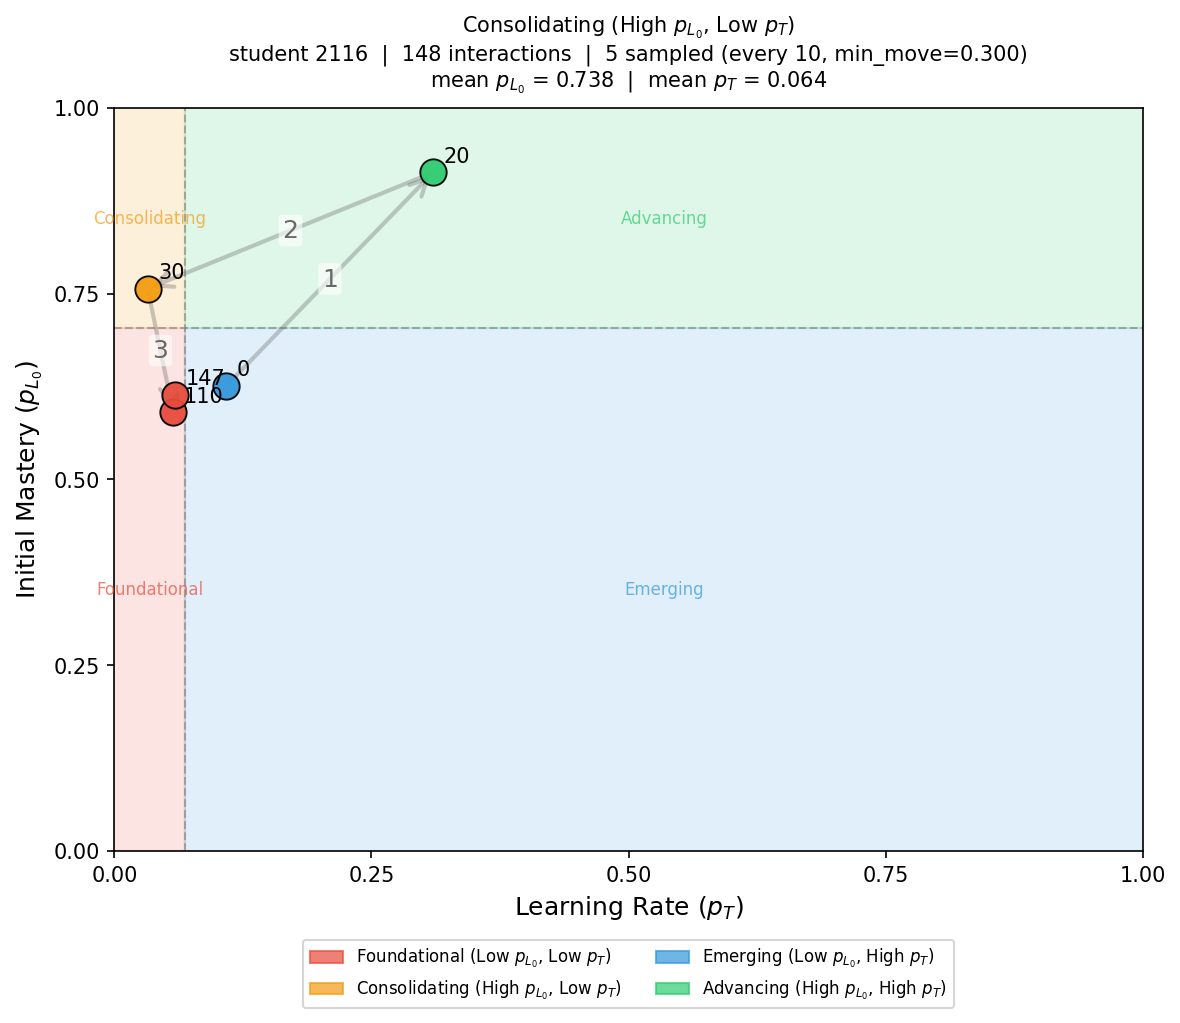
\includegraphics[width=0.8\textwidth,height=0.36\textheight,keepaspectratio]{roster_2d_consolidating_893468.png}
  \caption{\textit{Consolidating} (high $p_{L_0}$, low $p_T$): 3 points across 148 interactions. The trajectory is highly compact, remaining in the upper-left quadrant. The large marker at the final plotted point (interaction 25) encodes the remaining 123 interactions absorbed without a displacement exceeding $\delta_{\min}$: from that moment onward the student's parameter pair does not shift enough to register a new step. This prolonged absence of movement is the visible signal of stagnation; the instructional implication is to introduce novel or more challenging content to reactivate the learning trajectory.}
\end{subfigure}
\end{figure}
\begin{figure}[H]
\ContinuedFloat
\centering
\begin{subfigure}[b]{\textwidth}
  \centering
  
\includegraphics[width=0.8\textwidth,height=0.36\textheight,keepaspectratio]{roster_2d_emerging_893468.png}
  \caption{\textit{Emerging} (low $p_{L_0}$, high $p_T$): 15 points across 156 interactions (after removing 10 high-rate outliers). The trajectory is the most spatially extended of the four, crossing into all four quadrants over the course of the session. This wide variability is the defining feature of this learning situation: the student's profile is being actively revised at each interaction, signalling strong engagement and substantial growth potential. Sustained and progressively challenging practice is likely to consolidate the gains.}
\end{subfigure}
\begin{subfigure}[b]{\textwidth}
  \centering
  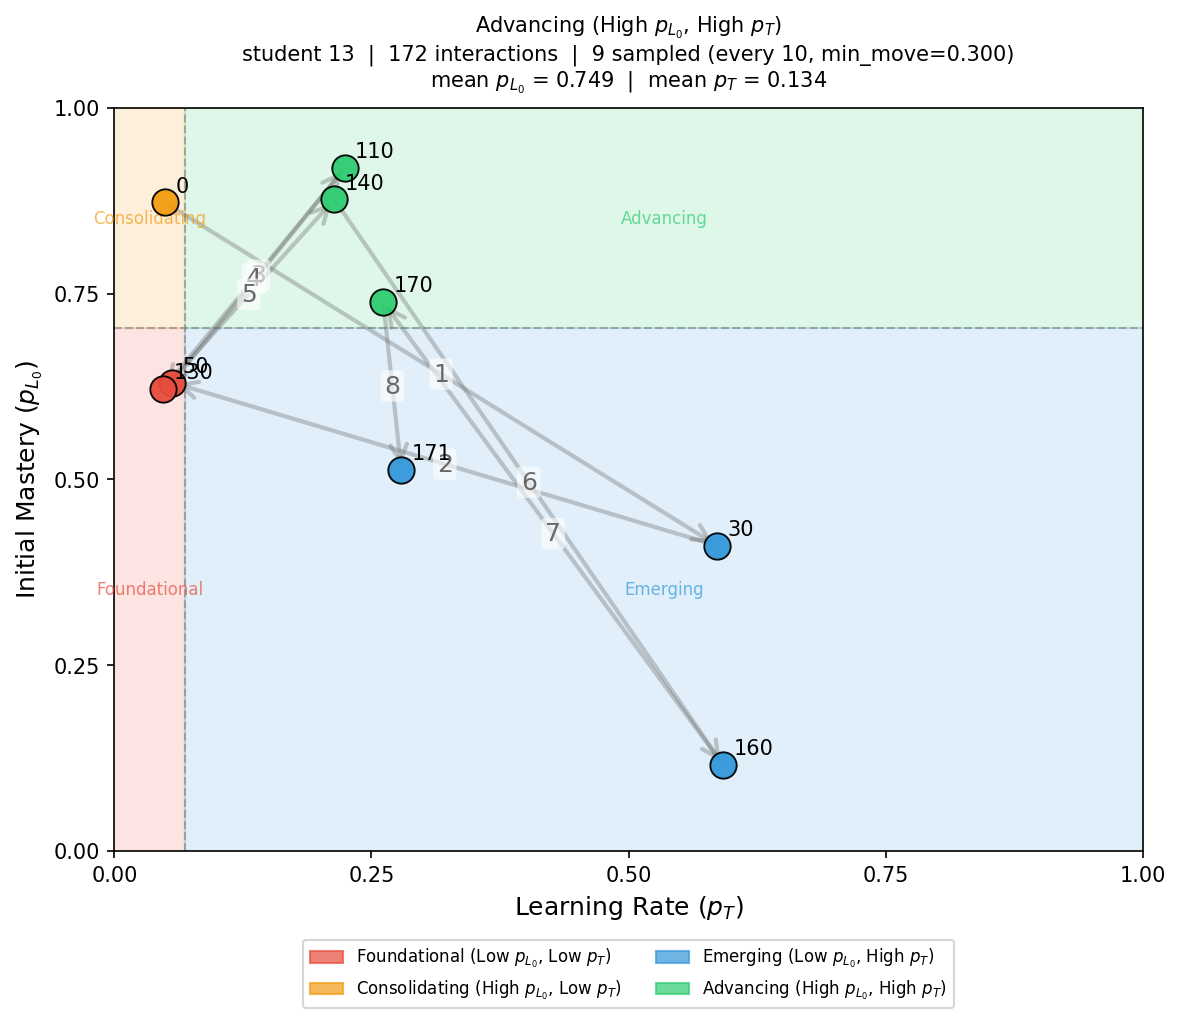
\includegraphics[width=0.8\textwidth,height=0.36\textheight,keepaspectratio]{roster_2d_advancing_893468.png}
  \caption{\textit{Advancing} (high $p_{L_0}$, high $p_T$): 4 points across 168 interactions. The trajectory consistently shows high prior mastery with above-median learning rates. The large marker at the final plotted point encodes the remaining interactions without sufficient displacement to register a new step, confirming that the parameter pair remains in the upper-right quadrant for most of the session. This pattern supports routing to accelerated or enriched content without risk of premature challenge.}
\end{subfigure}
\end{figure}

The parameter orbits of representative students across the four learning situations are characterised in Figures~\ref{fig_ellipse} and~\ref{fig_returnmap}. A key property of the augmented user model is that the learning situation assigned to each student is not a static category frozen at enrolment: it is a summary of the student's longitudinal tendency, continuously updated as new interactions arrive. The covariance ellipses in Figure~\ref{fig_ellipse} make this explicit: each ellipse visualises the full spread of $(p_{\text{L}_0}, p_{\text{T}})$ values that a student's profile traverses across all interactions, rather than a single point estimate.

For \textit{foundational} students, the ellipse is compact and centred at low mastery and low learning rate, indicating limited contextual variation: across skills and interactions, gTransformer consistently assigns this student low prior knowledge and a slow consolidation rate. This persistence is itself instructionally informative; the ellipse signals a structural mismatch between task demands and student preparation that calls for immediate scaffolding. Crucially, this diagnosis can be revised: if the student responds to the intervention and $p_{\text{L}_0}$ or $p_{\text{T}}$ begins to rise, the orbit will shift and the learning situation label will update accordingly.

For \textit{consolidating} students, the ellipse is compact and located at high mastery and low learning rate. The small spread indicates a stable region of the parameter space with little contextual variation: prior knowledge is high but the per-interaction learning rate has converged to near zero. The tutorial model should interpret this as a cue to introduce novel, cross-domain challenge or to advance the student to a higher difficulty tier, as continued practice at the current level is unlikely to produce further gains.

For \textit{emerging} students, the ellipse is the most spatially extended of all four situations, oriented along both the mastery and learning-rate axes. This broad orbit reflects a student whose parameters vary substantially across skills and contexts: at some skills the student is already proficient; at others, they are still building foundations with a high and increasing learning rate. The tutorial model should exploit this heterogeneity by differentiating at the skill level, rather than applying a uniform strategy to the whole student.

For \textit{advancing} students, the ellipse is moderately extended and centred at high mastery with a moderate learning rate. The spread confirms that the high-mastery profile is robust across contexts and not an artefact of easy items. The tutorial model can route this student to accelerated content and reduced practice redundancy.

\begin{figure}[H]
\caption{\textbf{Parameter orbit ellipses.} Covariance ellipses (1$\sigma$ and 2$\sigma$) for the representative student of each learning situation in $(p_{\text{L}_0}, p_{\text{T}})$ space. The centre marks the mean parameter position; ellipse shape encodes the extent and orientation of parameter variability across all interactions.}
\label{fig_ellipse}
\centering
\begin{subfigure}[b]{\textwidth}
  \centering
  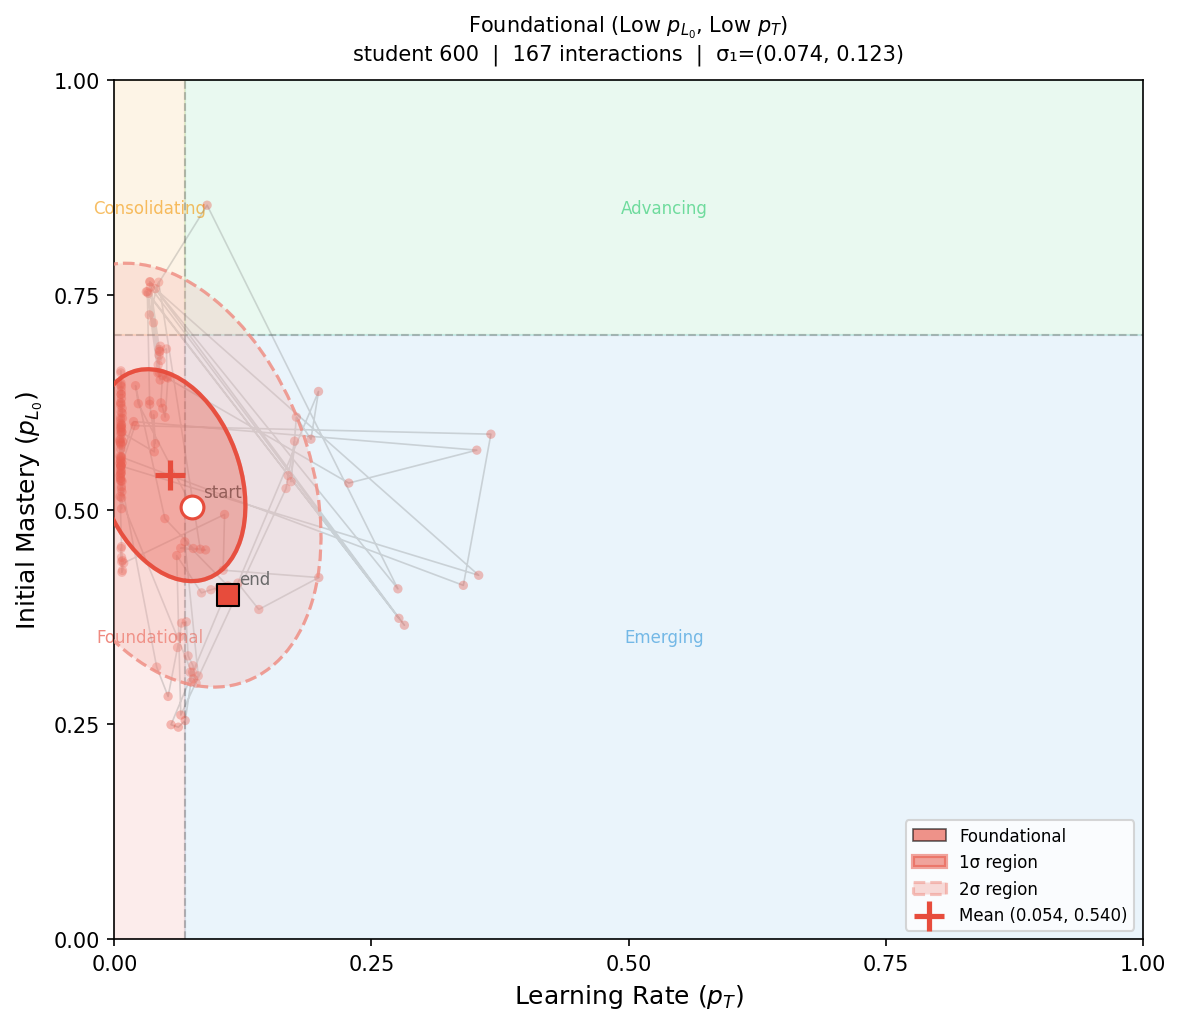
\includegraphics[width=0.8\textwidth,height=0.38\textheight,keepaspectratio]{attractor_ellipse_foundational_893468.png}
  \caption{\textit{Foundational} (low $p_{L_0}$, low $p_T$): compact ellipse at low mastery and low learning rate; persistent difficulty calls for immediate scaffolding.}
\end{subfigure}
\begin{subfigure}[b]{\textwidth}
  \centering
  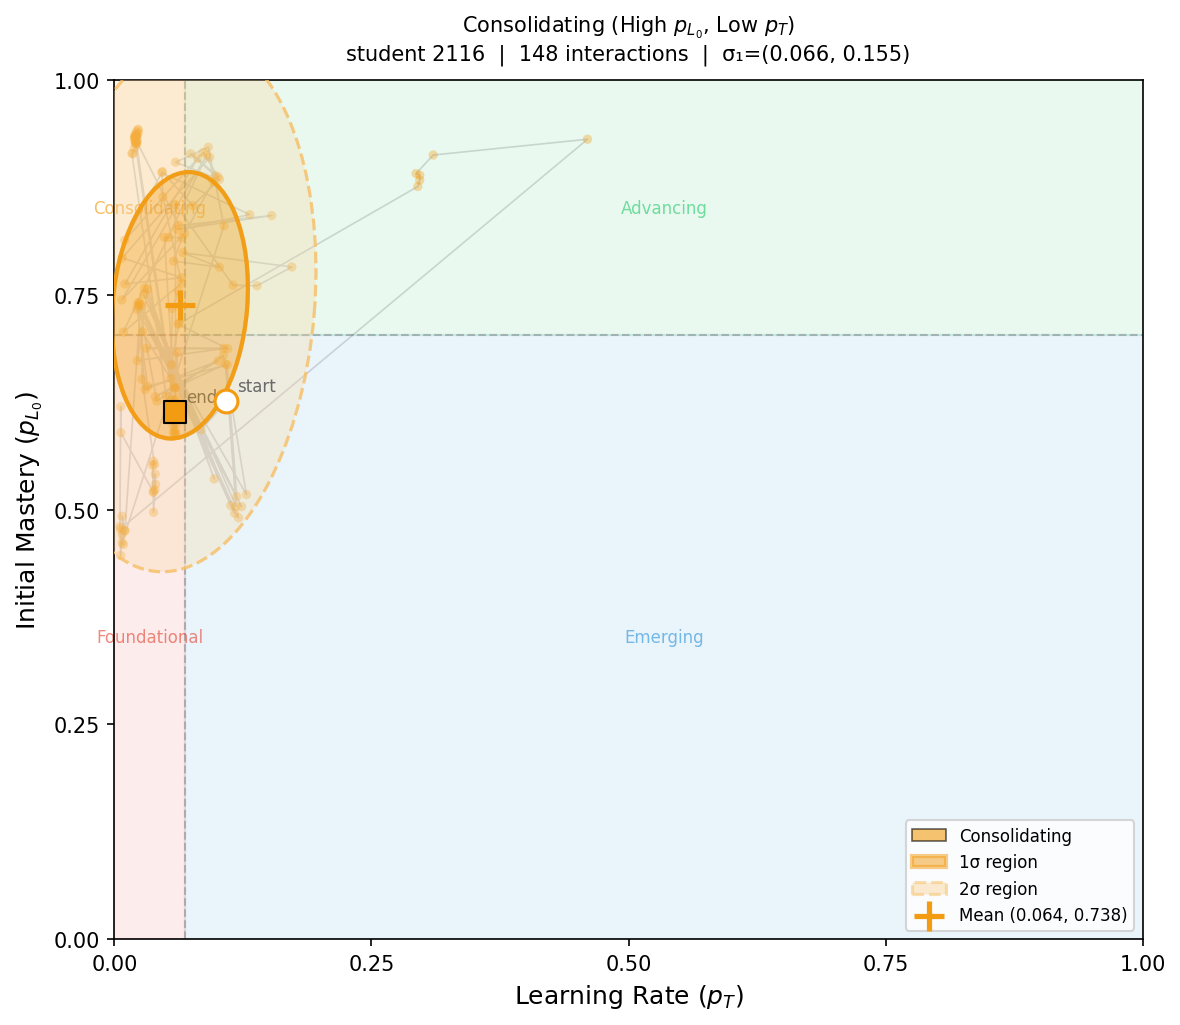
\includegraphics[width=0.8\textwidth,height=0.38\textheight,keepaspectratio]{attractor_ellipse_consolidating_893468.png}
  \caption{\textit{Consolidating} (high $p_{L_0}$, low $p_T$): compact ellipse at high mastery and near-zero learning rate; stagnation calls for novel challenge.}
\end{subfigure}
\end{figure}
\begin{figure}[H]
\ContinuedFloat
\centering
\begin{subfigure}[b]{\textwidth}
  \centering
  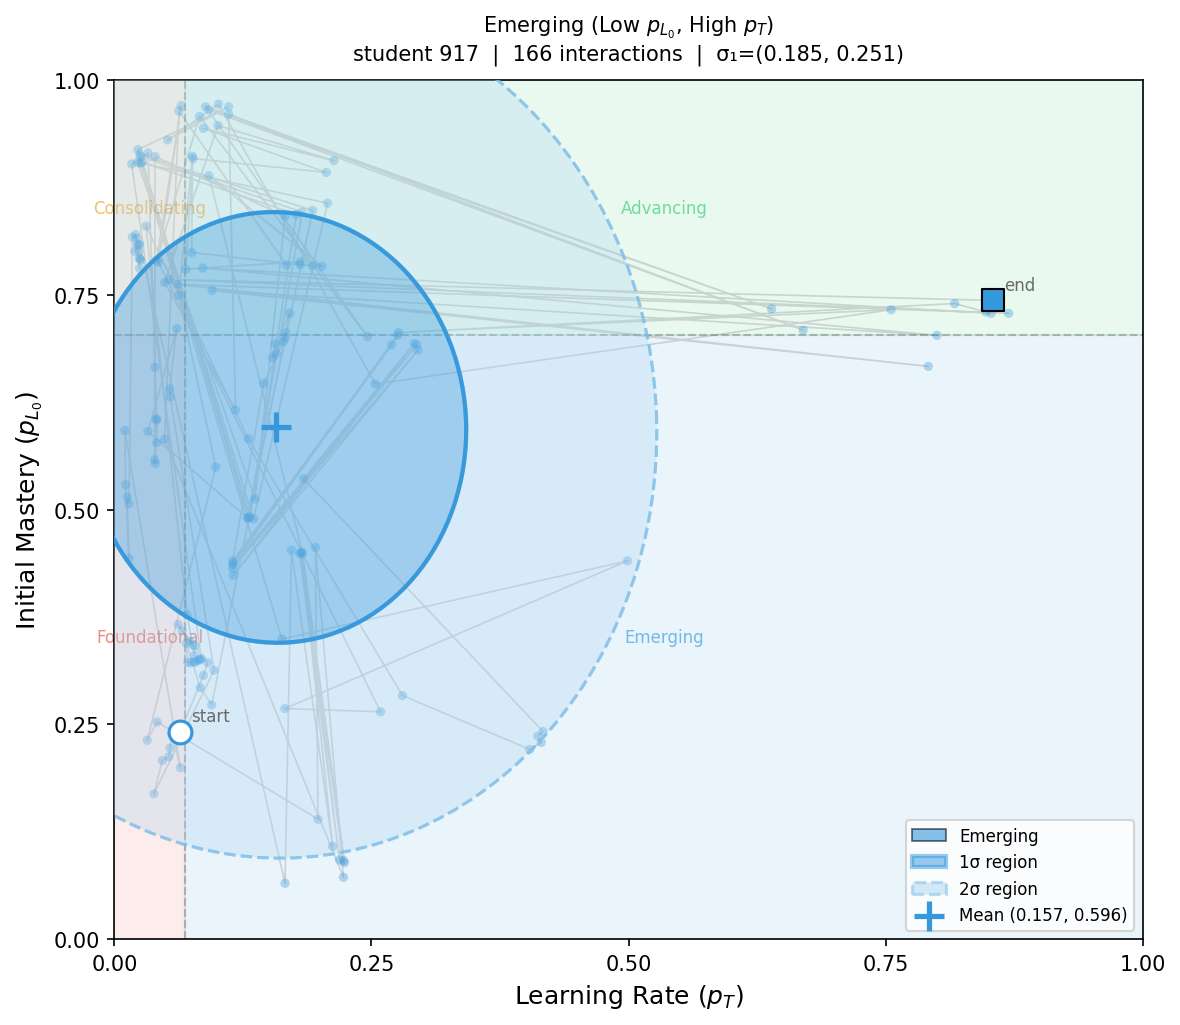
\includegraphics[width=0.8\textwidth,height=0.38\textheight,keepaspectratio]{attractor_ellipse_emerging_893468.png}
  \caption{\textit{Emerging} (low $p_{L_0}$, high $p_T$): most spatially extended ellipse; heterogeneous profile across skills benefits from skill-level differentiation.}
\end{subfigure}
\begin{subfigure}[b]{\textwidth}
  \centering
  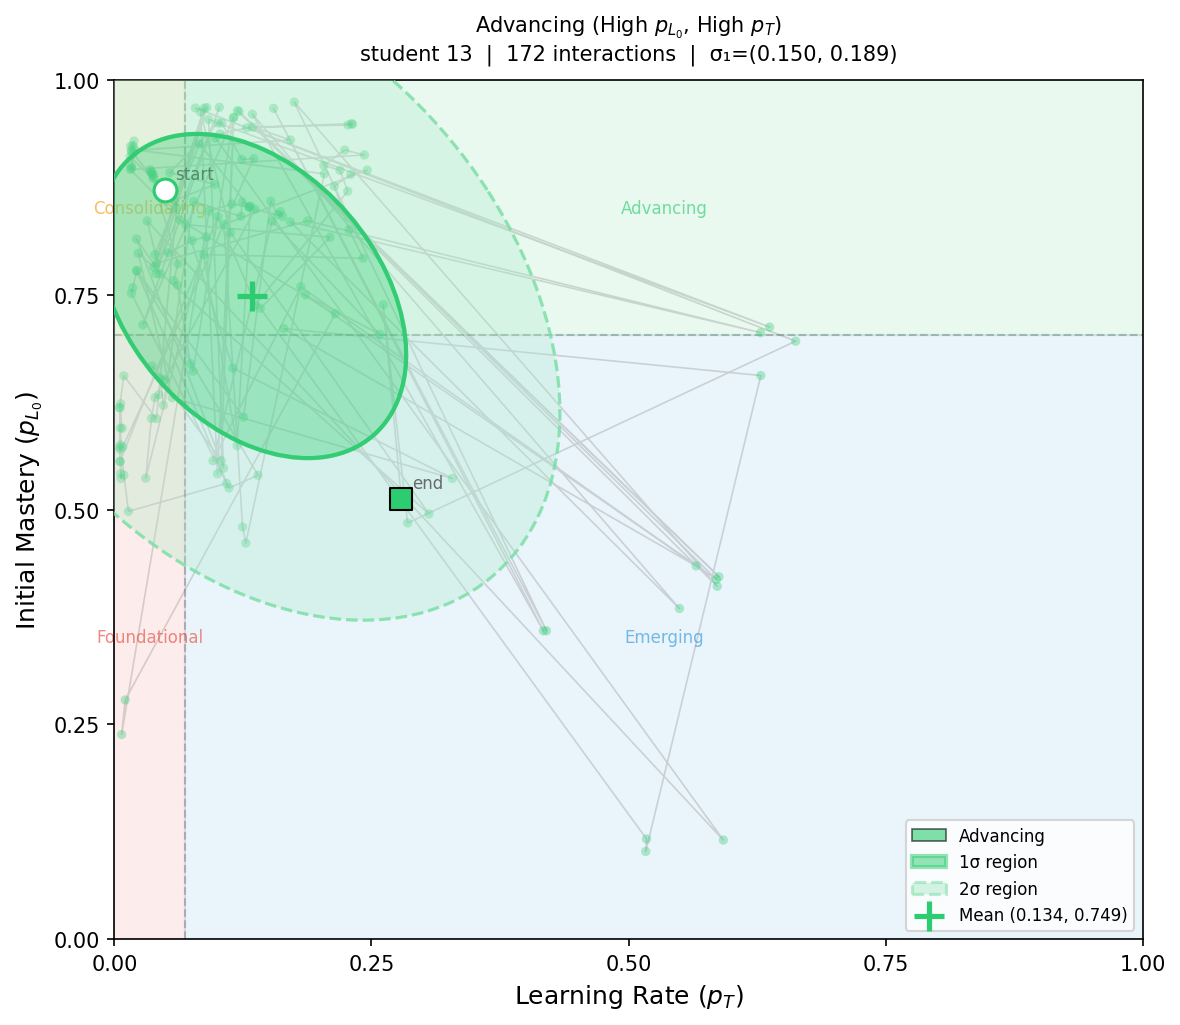
\includegraphics[width=0.8\textwidth,height=0.38\textheight,keepaspectratio]{attractor_ellipse_advancing_893468.png}
  \caption{\textit{Advancing} (high $p_{L_0}$, high $p_T$): moderately extended ellipse at high mastery and robust learning rate; supports routing to accelerated content.}
\end{subfigure}
\end{figure}

Figure~\ref{fig_returnmap} shows return maps for the same four representatives. Each panel plots the value of a parameter at interaction $t+1$ against its value at interaction $t$, separately for $p_{\text{L}_0}$ (left sub-panel) and $p_{\text{T}}$ (right sub-panel), with points coloured from dark (early interactions) to bright (late interactions). The diagonal represents a fixed point: points on the diagonal indicate no change between consecutive interactions. Deviations above the diagonal signal an increasing parameter; deviations below signal a decrease. Unlike population-level BKT, which produces a single pair of constant parameter values for all students on a given skill, each return map encodes the unique temporal trajectory of an individual student, a view that is both dynamic and context-aware.

For \textit{foundational} students, the $p_{\text{L}_0}$ return map reveals a systematic downward drift from early interactions (mean 0.61) to late interactions (mean 0.48): the model progressively revises its mastery estimate downward as evidence of insufficient learning accumulates. The $p_{\text{T}}$ panel is tightly concentrated near zero throughout, exposing a converging low-rate attractor. This temporal structure informs instructional timing: an intervention delivered before the orbit locks into the low attractor is far more likely to dislodge the student from this trajectory than one applied after convergence.

For \textit{consolidating} students, the $p_{\text{L}_0}$ return map undergoes a visible temporal transformation: early points span the mid range, while late points consolidate near the diagonal at high mastery (0.80). Simultaneously, $p_{\text{T}}$ declines from 0.077 to 0.050, converging toward a low-rate fixed point. The return map preserves the history of this transition, revealing that the student arrived at the plateau through accumulated practice. The tutorial model can exploit this information to introduce transferable challenge before the orbit fully stabilises.

For \textit{emerging} students, both $p_{\text{L}_0}$ (0.52 $\to$ 0.67) and $p_{\text{T}}$ (0.12 $\to$ 0.20) increase over time, with points distributed above the diagonal in both panels. The dynamic profile captures both early and late states and the transition between them, enabling the tutorial model to progressively accelerate pacing matched to the observed trajectory rather than to a predetermined category.

For \textit{advancing} students, the $p_{\text{L}_0}$ return map shows early stabilisation: mastery is high from the first interactions (mean 0.74) and clusters near the diagonal. The $p_{\text{T}}$ panel declines moderately (0.15 $\to$ 0.11), indicating diminishing marginal gains. The tutorial model can route this student to more demanding content immediately, grounded in the observed trajectory.

\begin{figure}[H]
\caption{\textbf{Return maps.} Plots for the representative student of each learning situation. Each panel shows $p_{\text{L}_0}(t+1)$ vs $p_{\text{L}_0}(t)$ (left) and $p_{\text{T}}(t+1)$ vs $p_{\text{T}}(t)$ (right). Points are coloured from dark (early) to bright (late) interactions. The diagonal (dashed line) marks the fixed point; deviations above indicate increasing parameters and deviations below indicate decreasing ones.}
\label{fig_returnmap}
\centering
\begin{subfigure}[b]{\textwidth}
  \centering
  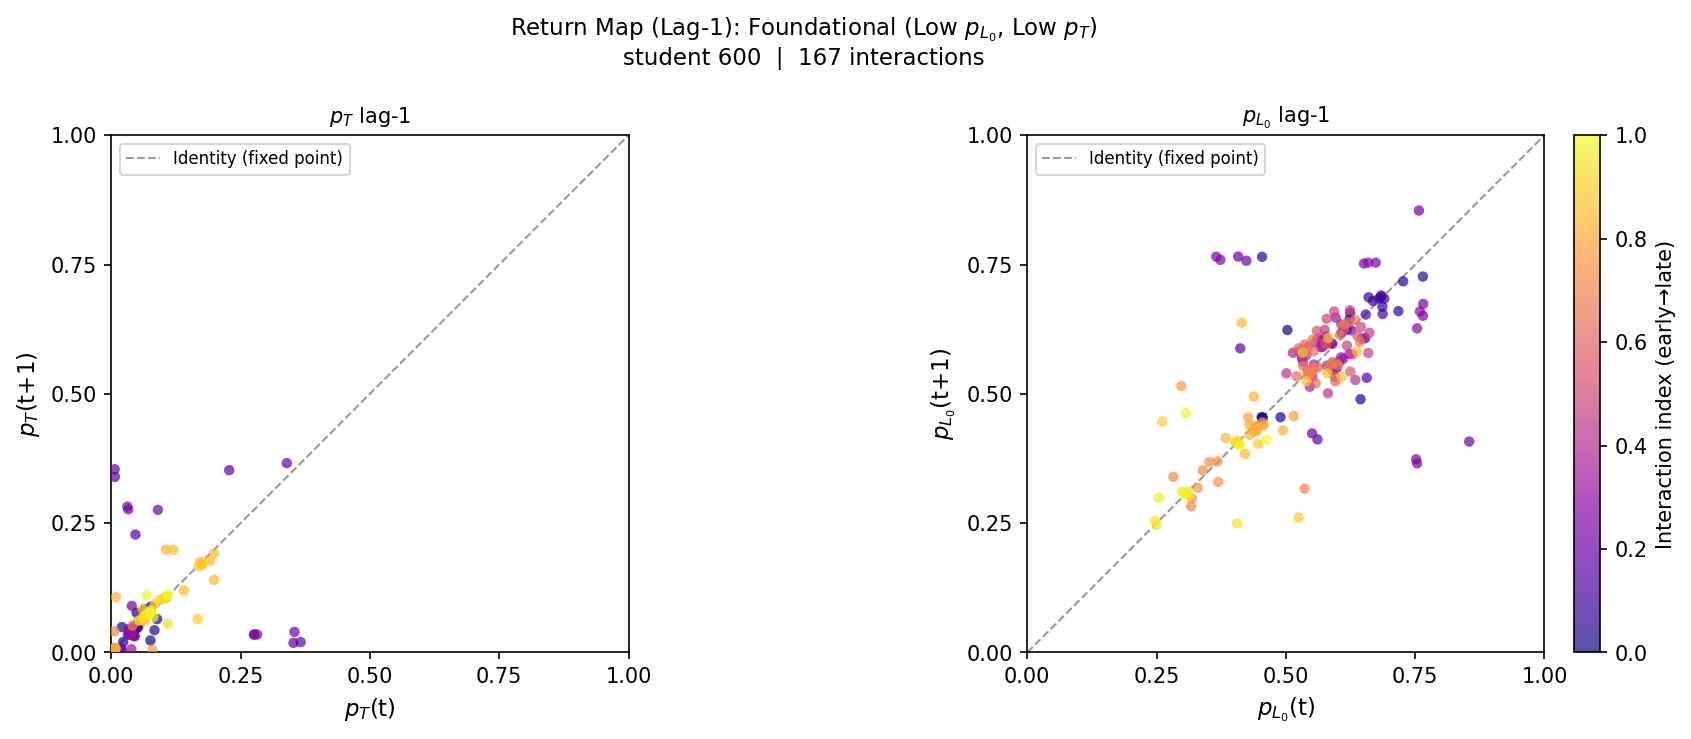
\includegraphics[width=0.9\textwidth,height=0.44\textheight,keepaspectratio]{attractor_returnmap_foundational_893468.png}
  \caption{\textit{Foundational} (low $p_{L_0}$, low $p_T$): broad scatter with downward mastery drift and a stable low learning-rate attractor converging over time.}
\end{subfigure}
\begin{subfigure}[b]{\textwidth}
  \centering
  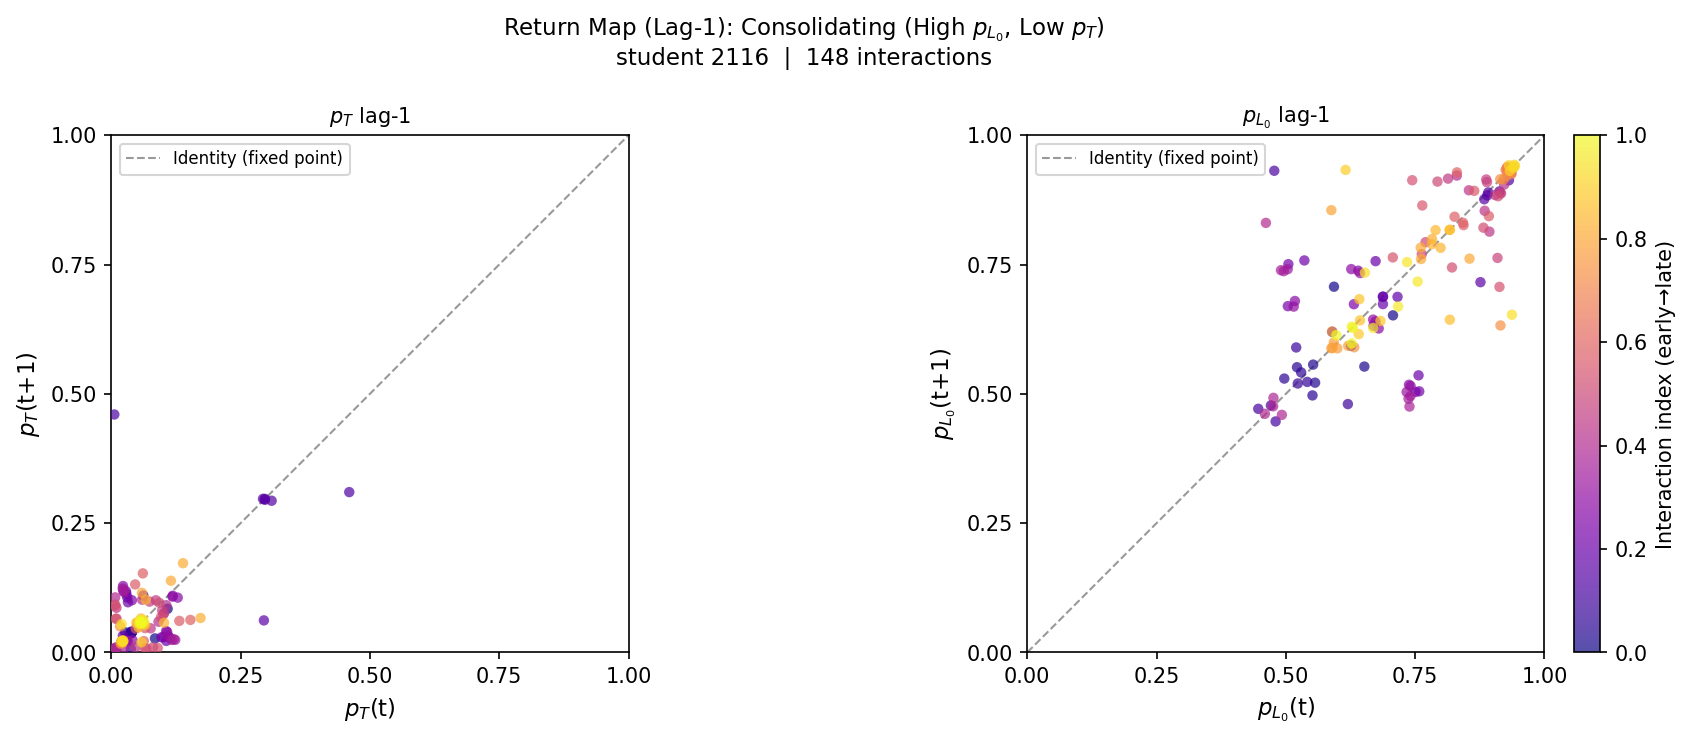
\includegraphics[width=0.9\textwidth,height=0.44\textheight,keepaspectratio]{attractor_returnmap_consolidating_893468.png}
  \caption{\textit{Consolidating} (high $p_{L_0}$, low $p_T$): mastery orbit migrates to a high-mastery fixed point while learning rate declines, revealing an active-to-plateau transition.}
\end{subfigure}
\end{figure}
\begin{figure}[H]
\ContinuedFloat
\centering
\begin{subfigure}[b]{\textwidth}
  \centering
  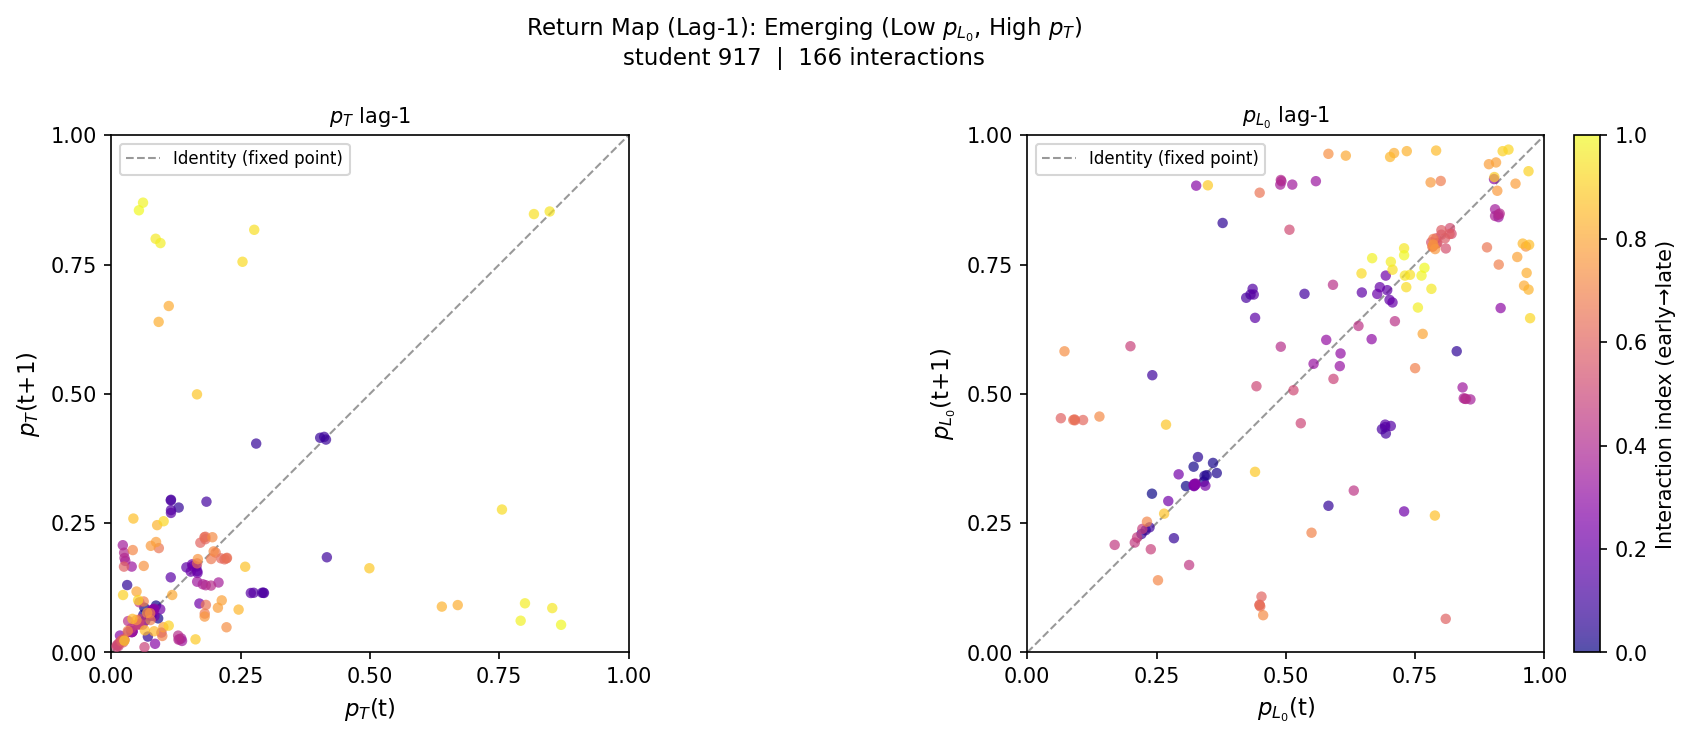
\includegraphics[width=0.9\textwidth,height=0.44\textheight,keepaspectratio]{attractor_returnmap_emerging_893468.png}
  \caption{\textit{Emerging} (low $p_{L_0}$, high $p_T$): both mastery and learning rate increase over time, with points distributed above the diagonal in both panels.}
\end{subfigure}
\begin{subfigure}[b]{\textwidth}
  \centering
  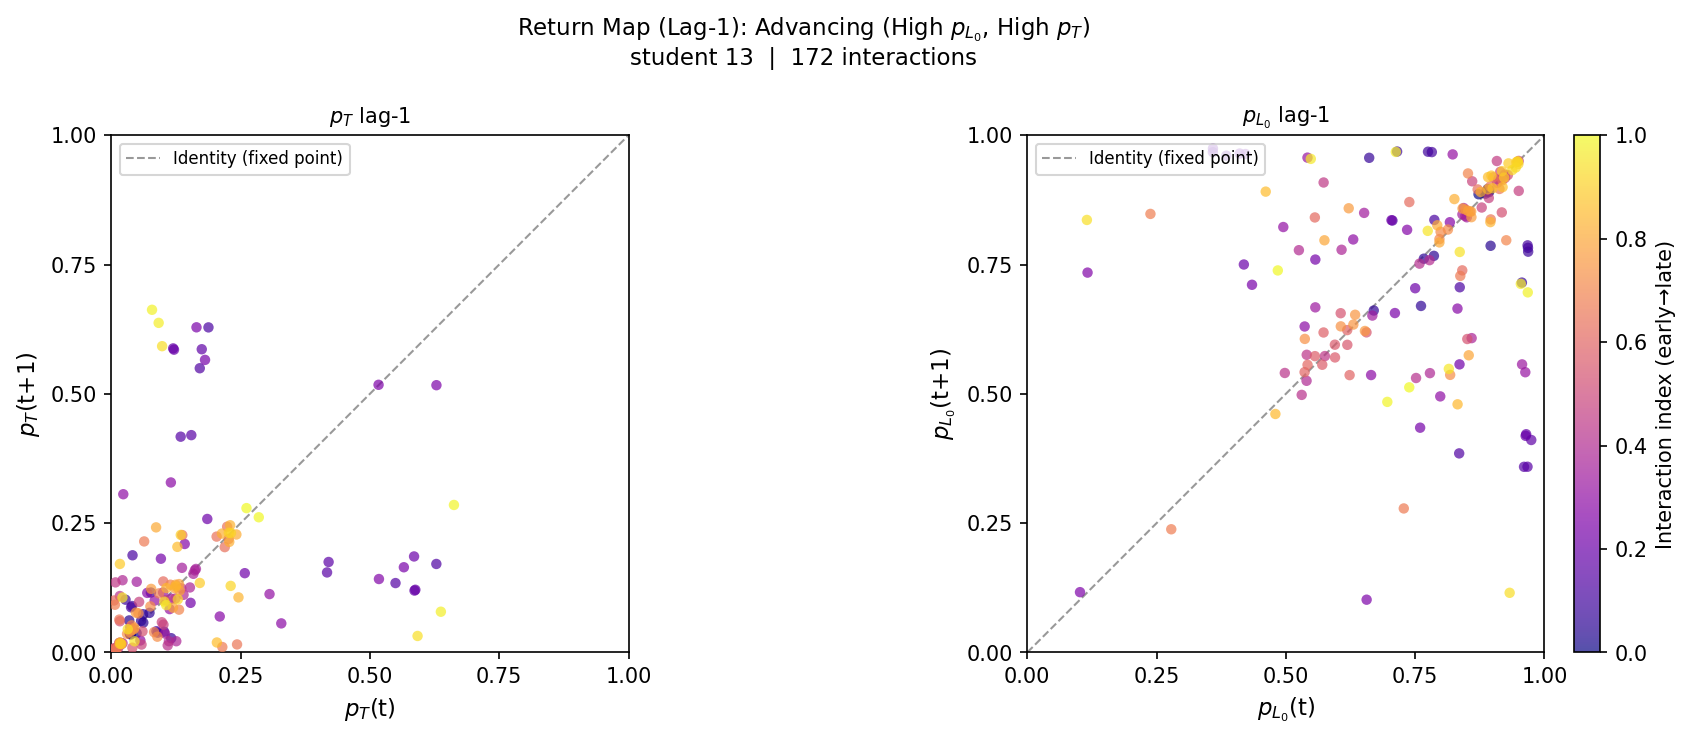
\includegraphics[width=0.9\textwidth,height=0.44\textheight,keepaspectratio]{attractor_returnmap_advancing_893468.png}
  \caption{\textit{Advancing} (high $p_{L_0}$, high $p_T$): mastery clusters at high values from the first interactions; learning rate declines moderately as marginal gains diminish.}
\end{subfigure}
\end{figure}

%
\section{Context-Aware Personalisation}
\label{sec_personalisation}

A key contribution of this work is demonstrating how the augmented student model enables the ITS tutorial model to move from population-level strategies towards situation-based, context-aware instruction. Rather than assigning students to fixed groups, the model identifies four learning situations by partitioning the $(p_{\text{L}_0}, p_{\text{T}})$ parameter space along two dimensions (prior knowledge and learning rate) on the AS2009 dataset. These learning situations are not static: because gTransformer continuously updates its parameter estimates as new interactions arrive, a student's assigned situation evolves with their trajectory. Each situation calls for a distinct tutorial strategy: students in the foundational situation require targeted scaffolding; those in the advancing situation are ready for accelerated pacing; intermediate situations benefit from adjusted challenge levels.

Each student interaction event can be routed to a different instructional pathway based on the current learning situation. A student whose trajectory places them in the foundational situation triggers a scaffolding strategy; a student identified as advancing is routed towards accelerated content progression. This routing is not static: as new interactions arrive, gTransformer updates its parameter estimates from the full longitudinal context, allowing the tutorial model to dynamically reassign students as their learning trajectory evolves. Two students with an identical recent response pattern may receive different instructional interventions if their prior histories place them in different learning situations, a distinction that population-level BKT cannot support.

Figure~\ref{fig_alluvial} illustrates the dynamic nature of these assignments. Of the 182 AS2009 students with at least 60 interactions, 67.0\% were assigned a different learning situation at session exit (last 30 interactions) versus session entry (first 30 interactions). This high transition rate confirms that the augmented model captures genuine learning dynamics rather than stable individual traits, and that situation-based routing responds to the student's observed trajectory rather than to a fixed initial categorisation.

%
\section{Discussion}

\subsection{Theory-Grounded Instructional Decisions}

The results demonstrate that augmenting the ITS student model with grounded Transformer parameters provides pedagogically meaningful differentiation at a minimal performance cost. The 19.9\% AUC gain over classical BKT confirms that student-specific, context-aware parameter estimates capture learning dynamics that population-level models cannot represent, while the low grounding cost (3.9\% relative to black-box architectures) confirms that interpretability is not purchased at a prohibitive predictive price.

By grounding instructional signals in BKT parameters ($p_{\text{L}_0}$, $p_{\text{T}}$) that practitioners recognise from established educational theory, the augmented student model provides educators with a diagnostic interface that neither classical BKT nor opaque deep learning models can offer. Decisions are traceable to constructs with pedagogical meaning; the tutorial model's routing recommendations can be inspected, questioned, and overridden by practitioners without requiring machine learning expertise.

\subsection{Beyond Static Labelling: Context-Aware Adaptation}

A central contribution of this design is the shift from population-level, static labelling to situation-based, dynamic diagnosis. The four learning situations are not fixed assignments: they are summaries of each student's current longitudinal profile, continuously revised as new interactions arrive. The 67\% session-level transition rate reported in Section~5 illustrates this directly: conditions that were foundational at session entry may become emerging or consolidating by session exit, and the tutorial model adapts its routing accordingly.

This dynamic property allows educators to identify, for instance, students in the consolidating situation (high prior knowledge but low learning rate, which may signal disengagement or instructional mismatch) and adapt the pacing before significant learning gaps emerge. Conversely, students in the advancing situation can be considered for accelerated progression to prevent unnecessary remediation. The design explicitly avoids treating learning situation labels as permanent characterisations of students: they describe observable learning patterns at a given point in time, not fixed attributes of the individual.

\subsection{Pedagogical Integrity and Educator Agency}

Triple-validation analyses reported in~\cite{labra2026theory} establish that gTransformer's internal representations genuinely encode BKT constructs as primary organising principles rather than as surface correlates. Structural alignment confirms that BKT constructs organise the latent space; semantic alignment confirms that grounded parameters retain their pedagogical semantics; and functional alignment quantifies the confidence with which educators can trust interpretable predictions. These properties mean that the learning situation labels derived from gTransformer are not arbitrary clusters: they reflect genuine differences in prior knowledge and learning rate detectable from the student's full interaction history.

This grounding in validated pedagogical constructs supports a specific form of educator agency: the practitioner can examine a student's parameter trajectory, understand why a learning situation was assigned, and decide whether and how to act. The system presents structured evidence; the instructional decision remains with the educator.

\subsection{Mindful TEL and Responsible AI}

The design presented in this paper is aligned with the ECTEL 2026 theme of Mindful TEL: Learning Technologies Shaped with Intention. Each design choice described in Section~2.3 reflects an explicit intention: interpretability is a first-class requirement, not a post hoc addition; transparency is directed at practitioners, not only AI specialists; and educator agency is preserved through deliberate constraints on automation. These are not rhetorical positions; they are instantiated in the model's architecture (grounded track, BKT parameter space), in the representation of its outputs (learning situation labels with defined instructional implications), and in its interaction model (decision support, not automated execution).

This approach is also responsive to the European regulatory context. The Artificial Intelligence Act (EU) 2024/1689 classifies AI systems that assess or monitor learners as high-risk, imposing requirements for transparency, human oversight, and accountability. The augmented student model addresses these requirements directly: its outputs are grounded in a well-established theoretical framework, its reasoning is traceable to parameters that educators can inspect, and its design explicitly reserves instructional decisions for human practitioners. By combining strong predictive performance with end-user interpretability, the model demonstrates that responsible deployment of AI in high-stakes educational contexts does not require sacrificing accuracy.

Limitations of the current design should be acknowledged. The learning situation partition uses a fixed threshold at the population median, which may not generalise uniformly across datasets with different score distributions. The model does not currently surface estimates of uncertainty to educators, which would strengthen the basis for human judgment. The augmented student model also does not address potential algorithmic biases that may arise if the BKT reference model was fitted on data that underrepresents certain student populations. These are directions for future work.

%
\section{Conclusions}

This paper contributes the design of an augmented student model for ITS that operationalises the principles of grounded Transformers into instructionally actionable representations, enabling educators to identify distinct learning situations and adapt instruction accordingly. Following the conceptual framework established in~\cite{labra2026theory}, we have shown how the continuously updated estimates of prior knowledge and learning rate produced by a grounded Transformer can be translated into a four-situation partition of the parameter space, each situation implying a concrete and theoretically grounded instructional strategy.

The results on the AS2009 dataset confirm both the predictive validity of the approach (19.9\% AUC gain over classical BKT) and the dynamic character of learning situation assignments (67.0\% of students assigned a different situation at session exit versus entry). The design is grounded in learning theory, transparency, and educator agency as first-class requirements, responding directly to the ECTEL 2026 theme of Mindful TEL and to the regulatory demands of the EU AI Act for high-risk educational AI systems.

The representational grounding methodology is domain-independent and may be extended to other theoretical frameworks beyond BKT. Future work will investigate the integration of uncertainty quantification into learning situation labels, the extension of the design to alternative learning theories, and the evaluation of the augmented student model in live ITS deployments with practitioner feedback.

%
\begin{figure}[H]
  \centering
  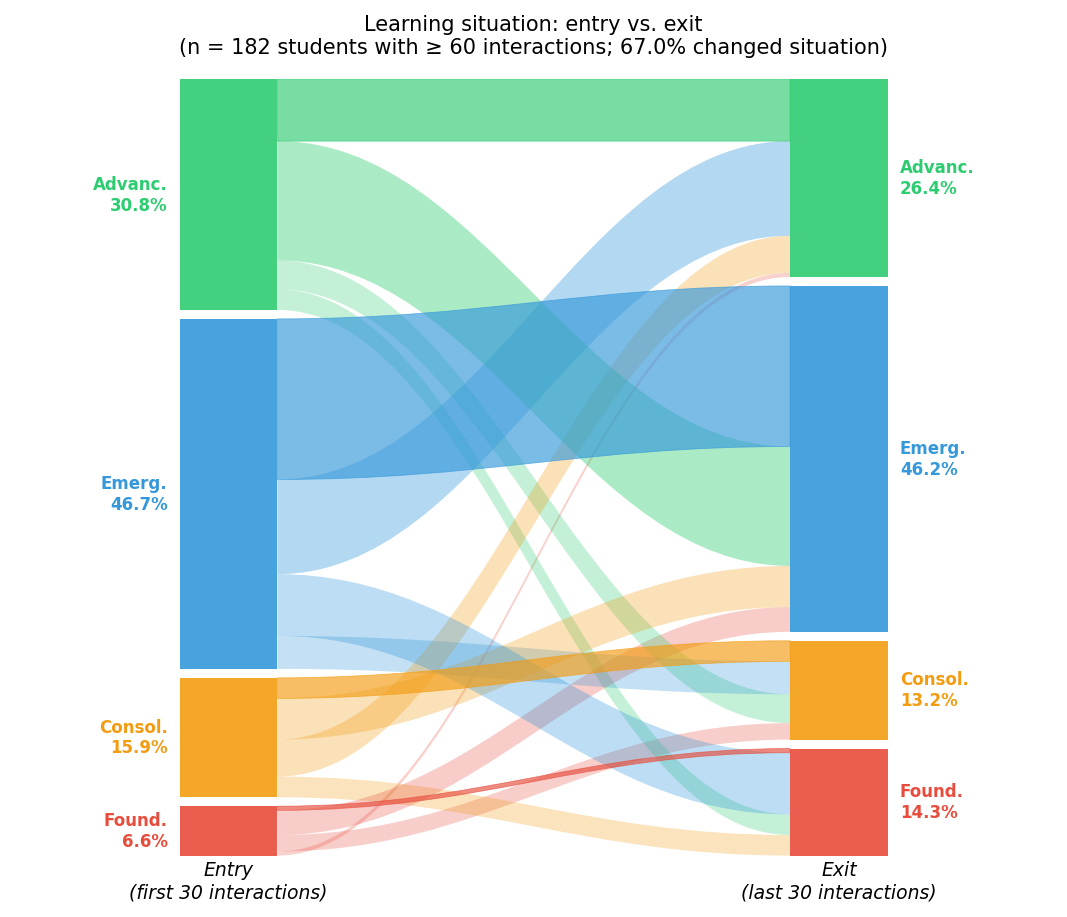
\includegraphics[width=0.75\textwidth,keepaspectratio]{situation_alluvial_893468.png}
  \caption{Learning situation at session entry (first 30 interactions) versus session exit (last 30 interactions) for $n = 182$ students with at least 60 interactions. Ribbon width is proportional to the fraction of students. Ribbons are coloured by entry situation; crossing ribbons indicate a change of learning situation over the course of the session. 67.0\% of students were assigned a different learning situation at the end of their session.}
  \label{fig_alluvial}
\end{figure}

\begin{figure}[H]
  \centering
  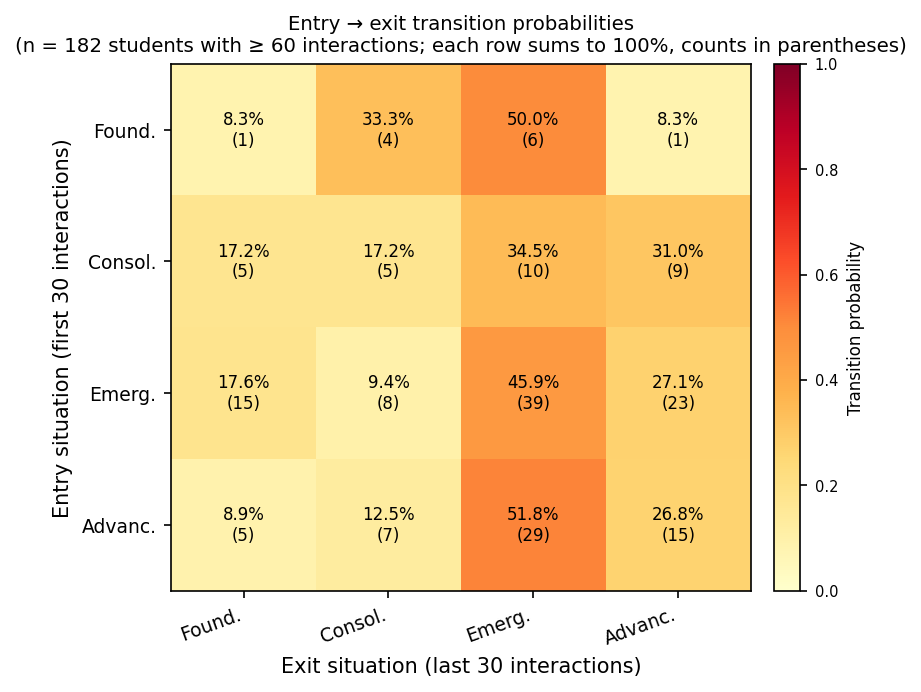
\includegraphics[width=0.55\textwidth,keepaspectratio]{situation_transition_matrix_893468.png}
  \caption{Entry-to-exit transition probabilities across the four learning situations ($n = 182$ students with at least 60 interactions; entry = first 30 interactions, exit = last 30 interactions). Each row sums to 100\%; raw student counts are shown in parentheses.}
  \label{fig_transition_matrix}
\end{figure}

%
\begin{credits}
\subsubsection{\ackname}
This research received no external funding.

\subsubsection{\discintname}
The authors have no competing interests to declare that are relevant to the content of this article.
\end{credits}

%
\bibliographystyle{splncs04cite}

\bibliography{biblio}

\end{document}
